\documentclass[serif]{beamer}
\input{sns_beamer_preamble.tex}
\usepackage{tikz-3dplot}

\begin{document}
\begin{frame}{위상수학에서는 대충 이런 걸 합니다}
    중등임용고시 수학 기출문제를 통해 위상수학을 아주 살짝 맛보는 시간을 가져보겠습니다.

    \begin{hint}[2026학년도 전공 A 12번]
        집합 $A=\{(x,y)\in\mathbb R^2\mid -1\leq x<1\}$ 위에서 거리함수 $d$를
        \[
            d((x,y),(x^\prime,y^\prime))=\min\left\{\sqrt{(x-(x^\prime+k))^2+(y-y^\prime)^2}\mid k=-2,0,2\right\}
        \]
        라 하자. 집합 $\biggl\{(x,0)\in A\mid d((-1,0),(x,0))\leq\dfrac{1}{2}\biggr\}$에 속하는 점의 $x$좌표 중 가장 작은 양의 실수를 풀이 과정과 함께 쓰시오.
        또한 $\mathbb R^2_*=\mathbb R^2-\{(0,0)\}$에 대하여 함수 $f:A\to\mathbb R^2_*$을 $f(x,y)=e^y(\cos\pi x,\sin\pi x)$라 하고, $\mathbb R^2_*$ 위에서 거리함수 $d_*$을
        \[
            d_*((u,v),(u^\prime,v^\prime))=d(f^{-1}(u,v),f^{-1}(u^\prime,v^\prime))
        \]
        이라 하자. 거리공간 $(\mathbb R^2_*,d_*)$에서 수열(sequence) $\biggl\{\biggl(0,\dfrac{1}{n}\biggr)\biggr\}$이 코시수열(Cauchy sequence)이 아님을 보이시오.
    \end{hint}
\end{frame}

\begin{frame}
    일단 적당히 풀어보겠습니다.
    \begin{hint}
        주어진 거리함수 $d$의 정의에 따라
        \[
            d((-1,0),(x,0))=\min\{\vert x-1\vert,\vert x+1\vert,\vert x+3\vert\}
        \]
        이므로 $d((-1,0),(x,0))\leq\dfrac{1}{2}$을 만족하는 가장 작은 양의 실수 $x$는 $\dfrac{1}{2}$입니다.
        \[
            f^{-1}\biggl(0,\frac{1}{n}\biggr)=\biggl(\frac{1}{2},-\ln n\biggr)
        \]
        임을 이용하면 자연수 $n$에 대하여
        \[
            d_*\biggl(\biggl(0,\frac{1}{n}\biggr),\biggl(0,\frac{1}{2n}\biggr)\biggr)=d\biggl(\biggl(\frac{1}{2},-\ln n\biggr),\biggl(\frac{1}{2},-\ln 2n\biggr)\biggr)=\ln 2
        \]
        이므로 주어진 수열은 코시수열이 아님을 알 수 있습니다.
    \end{hint}
    문제가 길어서 그렇지 어렵지는 않습니다. 정의만 잘 따라가면 됩니다. \\
    하지만 여기서 멈추면 수학도가 아닙니다. 좀 더 파고들어 봅시다.
\end{frame}


\begin{frame}
    \begin{hint}[일반화 시도하기]
        거리공간 $(A,d)$에서 점 $(-1,0)$을 중심으로 하고 반지름의 길이가 $\dfrac{1}{2}$인 열린 공
        \[
            B_d\biggl((-1,0),\frac{1}{2}\biggr)=\left\{(x,y)\in A~\middle\vert~d((-1,0),(x,y))<\frac{1}{2}\right\}
        \]
        을 좌표평면에 그림으로 나타내시오.
    \end{hint}
    평가원은 숫자를 아무렇게나 깔지 않습니다. 문제에서 주어진 점 $(-1,0)$은 집합 $A$의 경계에 위치하고 있습니다! 경계점에서의 열린 공의 모양을 살펴보고자 하는 욕구가 샘솟아야 합니다. \\
    정의로 다시 돌아갑시다.
    \[
        d((x,y),(x^\prime,y^\prime))=\min\left\{\sqrt{(x-(x^\prime+k))^2+(y-y^\prime)^2}\mid k=-2,0,2\right\}
    \]
    직관적으로 보면, 거리함수 $d$는 유클리드 거리를 약간 비틀어 $k\in\{-2,0,2\}$만큼 $x$축 방향으로의 평행이동을 허용하는 것과 같습니다. 즉, 우리는 점 $(-1,0)$을 반대편에 위치한 $(1,0)$과 일치시켜 생각할 수 있습니다.
    같은 방식으로 띠 모양의 공간 $A$의 왼쪽 경계(직선 $x=-1$)를 오른쪽 경계(직선 $x=1$)와 동일시할 수 있습니다. 이때 점 $(-1, y)$는 점 $(1,y)$에 대응됩니다. \\
    두 경계선을 일치시켰으므로 이어붙이는 조작이 가능합니다. 적당한 A4용지 한 장을 양손으로 들고 왼쪽 변과 오른쪽 변을 종이를 꼬지 않고 이어붙여 보세요!
\end{frame}

\begin{frame}
    앞에 글이 너무 많았네요. 그림으로 요약하겠습니다.
    \begin{figure}[H]
        \centering
        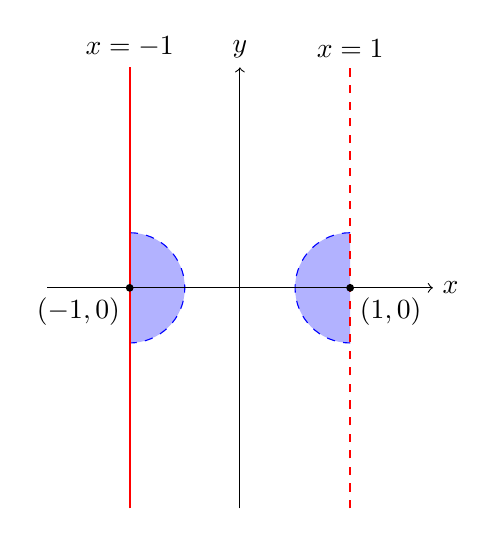
\begin{tikzpicture}[scale=0.7]
            \draw[dashed, draw=blue, fill=blue!30] (-2,1) arc (90:-90:1);
            \draw[dashed, blue, fill=blue!30] (2,1) arc (90:270:1);
            \draw[->] (-3.5,0) -- (3.5,0) node[right] {$x$};
            \draw[->] (0,-4) -- (0,4) node[above] {$y$};
            \draw[draw=red!100, thick] (-2,-4) -- (-2,4) node[above] {$x=-1$};
            \draw[dashed, thick, draw=red!100] (2,-4) -- (2,4) node[above] {$x=1$};
            \fill (-2,0) circle (2pt);
            \node[below left] at (-2,0) {$(-1,0)$};
            \fill (2,0) circle (2pt);
            \node[below right] at (2,0) {$(1,0)$};
        \end{tikzpicture}
        \quad
        \tdplotsetmaincoords{70}{97.5}
        \begin{tikzpicture}[tdplot_main_coords, scale=1.3]
            \def\R{1.4}       % 원통 반지름
            \def\H{2.0}       % 원통 반높이 (z = -H ~ H)
            \def\rball{0.6}   % 열린 공 반지름
            \def\thetaS{0}   % 봉합선 (x = -1 ~ 1) 위치 각도

            % 윗면 및 아랫면 원
            \tdplotdrawarc[gray!50, thin]{(0,0,\H)}{\R}{0}{360}{}{}
            \tdplotdrawarc[gray!50, thin]{(0,0,\H-1)}{\R}{0}{360}{}{}
            \tdplotdrawarc[gray!50, thin]{(0,0,0)}{\R}{0}{360}{}{}
            \tdplotdrawarc[gray!50, thin]{(0,0,-\H+1)}{\R}{0}{360}{}{}
            \tdplotdrawarc[gray!50, thin]{(0,0,-\H)}{\R}{0}{360}{}{}

            % 원통 외곽 기둥선
            \draw[gray!60, thin] ({\R*cos(45)}, {\R*sin(45)}, -\H) -- ({\R*cos(45)}, {\R*sin(45)}, \H);
            \draw[gray!60, thin] ({\R*cos(90)}, {\R*sin(90)}, -\H) -- ({\R*cos(90)}, {\R*sin(90)}, \H);
            \draw[gray!60, thin] ({\R*cos(135)}, {\R*sin(135)}, -\H) -- ({\R*cos(135)}, {\R*sin(135)}, \H);
            \draw[gray!60, thin] ({\R*cos(180)}, {\R*sin(180)}, -\H) -- ({\R*cos(180)}, {\R*sin(180)}, \H);
            \draw[gray!60, thin] ({\R*cos(225)}, {\R*sin(225)}, -\H) -- ({\R*cos(225)}, {\R*sin(225)}, \H);
            \draw[gray!60, thin] ({\R*cos(270)}, {\R*sin(270)}, -\H) -- ({\R*cos(270)}, {\R*sin(270)}, \H);
            \draw[gray!60, thin] ({\R*cos(315)}, {\R*sin(315)}, -\H) -- ({\R*cos(315)}, {\R*sin(315)}, \H);

            % 봉합선 표시
            \draw[red, thick] ({\R*cos(\thetaS)}, {\R*sin(\thetaS)}, -\H) -- ({\R*cos(\thetaS)}, {\R*sin(\thetaS)}, \H);

            % 원통 표면의 열린 공
            % 각도 범위(도 단위)
            \def\angleRange{25}

            % 근방 내부 영역 채우기
            \fill[blue!30, opacity=0.7]
                plot[domain=-\angleRange:\angleRange, samples=40] 
                ({ \R*cos(\thetaS + \x) }, 
                { \R*sin(\thetaS + \x) }, 
                { sqrt(max(0, \rball*\rball - (\R*\x*pi/180)^2)) })
                --
                plot[domain=\angleRange:-\angleRange, samples=40] 
                ({ \R*cos(\thetaS + \x) }, 
                { \R*sin(\thetaS + \x) }, 
                { -sqrt(max(0, \rball*\rball - (\R*\x*pi/180)^2)) })
                -- cycle;

            % 근방의 경계선
            \draw[dashed, blue!80!black, thick]
                plot[domain=-\angleRange:\angleRange, samples=40] 
                ({ \R*cos(\thetaS + \x) }, 
                { \R*sin(\thetaS + \x) }, 
                { sqrt(max(0, \rball*\rball - (\R*\x*pi/180)^2)) })
                --
                plot[domain=\angleRange:-\angleRange, samples=40] 
                ({ \R*cos(\thetaS + \x) }, 
                { \R*sin(\thetaS + \x) }, 
                { -sqrt(max(0, \rball*\rball - (\R*\x*pi/180)^2)) });

            % 중심점 및 레이블
            \fill[black] ({\R*cos(\thetaS)}, {\R*sin(\thetaS)}, 0) circle (1.2pt);
            \node[right] at ({\R*cos(\thetaS)+0.75}, {\R*sin(\thetaS)+2}, 0) {$(-1,0)$};
            \draw[->] ({\R*cos(\thetaS)+0.75}, {\R*sin(\thetaS)+2}, 0) -- ({\R*cos(\thetaS)+0.1}, {\R*sin(\thetaS)+0.1}, 0);
        \end{tikzpicture}
        \caption{좌: 거리공간 $A$, 우: 거리공간 $A$의 양 끝을 이어붙인 원통 공간 $S^1\times\mathbb R$}
    \end{figure}
    조금 엄밀하게 말하면, 공간 $A$는 원 $S^1$과 실수직선 $\mathbb R$의 곱공간 $S^1\times\mathbb R$과 위상동형입니다. 공간 $S^1\times\mathbb R$은 원이 무한히 길게 늘어선 말 그대로의 원통 모양의 공간입니다.
\end{frame}

\begin{frame}
    이제 공간 $S^1\times\mathbb R$을 보겠습니다. 여러분 손에 원통 모양으로 말려있는 A4 용지가 있다고 \\ 믿겠습니다. 여기서 약간의 상상력이 필요합니다.
    말려있는 A4 용지를 위에서 바라보고, \\ 원통의 옆면을 손으로 쭉 늘려서 평면에 원통을 이루는 각 원들이 놓이도록 해보세요. \\
    (머리속에서만 해보세요! 실제 종이는 찰흙처럼 늘릴 수 없다는 점을 기억하세요!)\\
    그러면 다음 그림과 같은 변형이 가능합니다.

    \begin{figure}[H]
        \centering
        \tdplotsetmaincoords{70}{97.5}
        \begin{tikzpicture}[tdplot_main_coords, scale=1.3]
            \def\R{1.4}       % 원통 반지름
            \def\H{2.0}       % 원통 반높이 (z = -H ~ H)
            \def\rball{0.6}   % 열린 공 반지름
            \def\thetaS{0}   % 봉합선 (x = -1 ~ 1) 위치 각도

            % 윗면 및 아랫면 원
            \tdplotdrawarc[gray!50, thin]{(0,0,\H)}{\R}{0}{360}{}{}
            \tdplotdrawarc[gray!50, thin]{(0,0,\H-1)}{\R}{0}{360}{}{}
            \tdplotdrawarc[gray!50, thin]{(0,0,0)}{\R}{0}{360}{}{}
            \tdplotdrawarc[gray!50, thin]{(0,0,-\H+1)}{\R}{0}{360}{}{}
            \tdplotdrawarc[gray!50, thin]{(0,0,-\H)}{\R}{0}{360}{}{}

            % 원통 외곽 기둥선
            \draw[gray!60, thin] ({\R*cos(45)}, {\R*sin(45)}, -\H) -- ({\R*cos(45)}, {\R*sin(45)}, \H);
            \draw[gray!60, thin] ({\R*cos(90)}, {\R*sin(90)}, -\H) -- ({\R*cos(90)}, {\R*sin(90)}, \H);
            \draw[gray!60, thin] ({\R*cos(135)}, {\R*sin(135)}, -\H) -- ({\R*cos(135)}, {\R*sin(135)}, \H);
            \draw[gray!60, thin] ({\R*cos(180)}, {\R*sin(180)}, -\H) -- ({\R*cos(180)}, {\R*sin(180)}, \H);
            \draw[gray!60, thin] ({\R*cos(225)}, {\R*sin(225)}, -\H) -- ({\R*cos(225)}, {\R*sin(225)}, \H);
            \draw[gray!60, thin] ({\R*cos(270)}, {\R*sin(270)}, -\H) -- ({\R*cos(270)}, {\R*sin(270)}, \H);
            \draw[gray!60, thin] ({\R*cos(315)}, {\R*sin(315)}, -\H) -- ({\R*cos(315)}, {\R*sin(315)}, \H);

            % 봉합선 표시
            \draw[red, thick] ({\R*cos(\thetaS)}, {\R*sin(\thetaS)}, -\H) -- ({\R*cos(\thetaS)}, {\R*sin(\thetaS)}, \H);

            % 원통 표면의 열린 공
            % 각도 범위(도 단위)
            \def\angleRange{25}

            % 근방 내부 영역 채우기
            \fill[blue!30, opacity=0.7]
                plot[domain=-\angleRange:\angleRange, samples=40] 
                ({ \R*cos(\thetaS + \x) }, 
                { \R*sin(\thetaS + \x) }, 
                { sqrt(max(0, \rball*\rball - (\R*\x*pi/180)^2)) })
                --
                plot[domain=\angleRange:-\angleRange, samples=40] 
                ({ \R*cos(\thetaS + \x) }, 
                { \R*sin(\thetaS + \x) }, 
                { -sqrt(max(0, \rball*\rball - (\R*\x*pi/180)^2)) })
                -- cycle;

            % 근방의 경계선
            \draw[dashed, blue!80!black, thick]
                plot[domain=-\angleRange:\angleRange, samples=40] 
                ({ \R*cos(\thetaS + \x) }, 
                { \R*sin(\thetaS + \x) }, 
                { sqrt(max(0, \rball*\rball - (\R*\x*pi/180)^2)) })
                --
                plot[domain=\angleRange:-\angleRange, samples=40] 
                ({ \R*cos(\thetaS + \x) }, 
                { \R*sin(\thetaS + \x) }, 
                { -sqrt(max(0, \rball*\rball - (\R*\x*pi/180)^2)) });

            % 중심점
            \fill[black] ({\R*cos(\thetaS)}, {\R*sin(\thetaS)}, 0) circle (1.2pt);
        \end{tikzpicture}
        \quad
        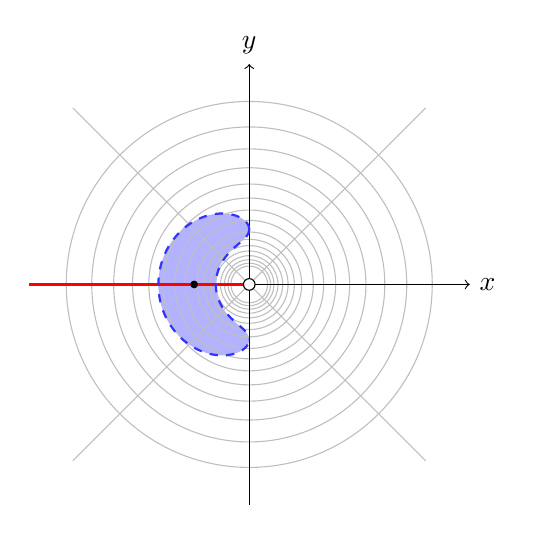
\begin{tikzpicture}[scale=0.7]
            \fill[blue!30]
            plot[domain=0:180, samples=360, variable=\t]
            ( {exp(sqrt(0.25 - ((\t-90)/180)^2)) * cos(\t+90)},
                {exp(sqrt(0.25 - ((\t-90)/180)^2)) * sin(\t+90)} )
            -- cycle;
            
            \fill[white]
            plot[domain=180:360, samples=360, variable=\t]
            ( {exp(-sqrt(0.25 - ((\t-270)/180)^2)) * cos(\t-90)},
                {exp(-sqrt(0.25 - ((\t-270)/180)^2)) * sin(\t-90)} );
        
            \foreach \j in {1,...,8}
                {
                    \draw[gray!50] (0,0) circle ({exp(0.15*\j)});
                    \draw[gray!50] (0,0) circle ({exp(-0.15*\j+0.1)});
                }
            \draw[draw=gray!50] (3.2,3.2) -- (-3.2,-3.2);
            \draw[draw=gray!50] (-3.2,3.2) -- (3.2,-3.2);
            \draw[draw=red, thick] (0,0) -- (-4,0);
            \draw[->] (0,0) -- (4,0) node[right] {$x$};
            \draw[->] (0,-4) -- (0,4) node[above] {$y$};
            \draw[fill=white] (0,0) circle (3pt);
            \fill (-1,0) circle (2pt);

            \draw[blue!80, dashed, thick]
                plot[domain=0:180, samples=360, variable=\t]
                ( {exp(sqrt(0.25 - ((\t-90)/180)^2)) * cos(\t+90)},
                    {exp(sqrt(0.25 - ((\t-90)/180)^2)) * sin(\t+90)} );

            \draw[blue!80, dashed, thick]
                plot[domain=180:360, samples=360, variable=\t]
                ( {exp(-sqrt(0.25 - ((\t-270)/180)^2)) * cos(\t-90)},
                    {exp(-sqrt(0.25 - ((\t-270)/180)^2)) * sin(\t-90)} );
        \end{tikzpicture}
        \caption{좌: 원통 $S^1\times\mathbb R$, 우: 구멍난 평면 $\mathbb R^2_*$}
    \end{figure}
    따라서 직관적으로 원통 $S^1\times\mathbb R$과 구멍난 평면 $\mathbb R^2_*=\mathbb R^2-\{(0,0)\}$은 위상동형입니다. \\
    주의: 여기서 $\mathbb R^2_*$은 평면 $\mathbb R^2$의 부분공간이 아니라, 거리공간 $(\mathbb R^2_*,d_*)$입니다.
\end{frame}

\begin{frame}
    사실 문제에서 주어진 함수 $f$를 보자마자 $A$와 $\mathbb R^2_*$이 위상동형임을 눈치채야 합니다.
    그래서 문제를 조금 더 어렵게 낼 작정이었으면 코시수열 여부를 직접 추론 하게끔 했을 겁니다.

    \begin{figure}[H]
        \centering
        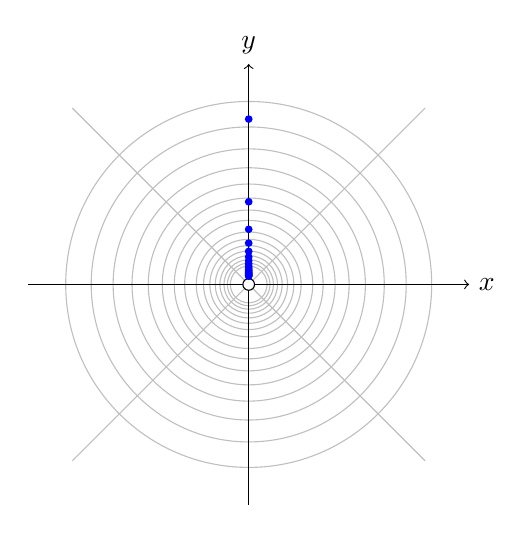
\begin{tikzpicture}[scale=0.7]
            \foreach \j in {1,...,8}
                {
                    \draw[gray!50] (0,0) circle ({exp(0.15*\j)});
                    \draw[gray!50] (0,0) circle ({exp(-0.15*\j+0.1)});
                }
            \draw[draw=gray!50] (3.2,3.2) -- (-3.2,-3.2);
            \draw[draw=gray!50] (-3.2,3.2) -- (3.2,-3.2);
            \draw[->] (-4,0) -- (4,0) node[right] {$x$};
            \draw[->] (0,-4) -- (0,4) node[above] {$y$};
            \draw[fill=white] (0,0) circle (3pt);
            
            \foreach \i in {1,...,20}
                {\fill[blue] (0,3/\i) circle (2pt);}
        \end{tikzpicture}
        \quad
        \begin{tikzpicture}[scale=0.7]
            \draw[->] (-4,0) -- (4,0) node[right] {$x$};
            \draw[->] (0,-4) -- (0,4) node[above] {$y$};
            \draw[draw=red!100, thick] (-2,-4) -- (-2,4) node[above] {$x=-1$};
            \draw[dashed, thick, draw=red!100] (2,-4) -- (2,4) node[above] {$x=1$};
            \draw[dashed, thick] (1,4) -- (1,-4);

            \foreach \i in {1,...,50}
                {\fill[blue] (1,{-ln(\i)}) circle (2pt);}
        \end{tikzpicture}
        \caption{좌: $\mathbb R^2_*$에서 수열 $\{(0,1/n)\}$, 우: $A$에서 수열 $\{(1/2,-\ln n)\}$}
    \end{figure}
    주어진 수열 역시 그림으로 나타내면 다음과 같습니다. $A$의 점들이 아래쪽으로 무한히 뻗어나간다는 사실에 유의하세요!
    (그림에서는 수렴하는 것처럼 보일 뿐, 실제로는 발산합니다.)
\end{frame}

\begin{frame}
    이제 지금까지 언급한 내용을 엄밀하게 증명할 차례입니다!
    \begin{prob*}{}
        평면 $\mathbb R^2$ 위에 동치 관계 $\sim$을 다음과 같이 정의하자.
        \[
            (x,y)\sim(x^\prime,y^\prime)~\Longleftrightarrow~x-x^\prime\in 2\mathbb Z\text{이고 } y=y^\prime
        \]
        이 동치 관계로 생성되는 몫공간(quotient space) $\mathbb R^2/\sim$을 생각하자.
        \begin{enumerate}[(a)]
            \item 거리공간 $(A,d)$가 몫공간 $\mathbb R^2/\sim$와 위상동형임을 보여라.
            \item 몫공간 $\mathbb R^2/\sim$이 곱공간 $S^1\times\mathbb R$과 위상동형임을 보여라.
            \item 거리공간 $(\mathbb R^2_*,d_*)$는 완비 거리 공간인가? 즉 임의의 코시수열이 수렴하는가?
        \end{enumerate}
    \end{prob*}
\end{frame}
\end{document}